\documentclass[10pt]{article}
\usepackage[utf8]{inputenc}
\usepackage[english]{babel}
\usepackage{multicol}
\usepackage{amssymb}
\usepackage{amsfonts}
\usepackage[bookmarks]{hyperref}
\usepackage[a4paper, total={18cm, 25cm}]{geometry}
\usepackage{graphicx}
\usepackage{xcolor}
\usepackage{textcomp}
\graphicspath{ {.} }
\usepackage{listings}
\usepackage{makecell}
\usepackage{qtree}
\usepackage{pgfplots}
\usepackage{tikz}
\usepackage{float}
\usetikzlibrary{quantikz, shapes, arrows}
\usepackage{blochsphere}
\usepgflibrary{shapes}
\usepackage{cancel}
\usepgfplotslibrary{fillbetween}
\definecolor{backcolour}{RGB}{255,255,255}
\definecolor{codegreen}{RGB}{27,168,11}
\definecolor{codeblue}{RGB}{35,35,205}
\definecolor{codegray}{RGB}{128,128,128}
\definecolor{codepurple}{RGB}{205,35,56}
\lstdefinestyle{myPython}{
	backgroundcolor=\color{backcolour},   
	commentstyle=\color{codegreen},
	keywordstyle=\color{codeblue},
	numberstyle=\tiny\color{codegray},
	stringstyle=\color{codepurple},
	basicstyle=\small\ttfamily,
	breakatwhitespace=false,         
	breaklines=true,                 
	captionpos=b,                    
	keepspaces=true,                 
	numbers=left,                    
	numbersep=2pt,                  
	showspaces=false,                
	showstringspaces=false,
	showtabs=false,                  
	tabsize=2,
	language=python
}
\newcommand*\triangled[1]{\tikz[baseline=(char.base)]{
            \node[regular polygon, regular polygon sides=3,draw,inner sep=1pt] (char) {#1};}}
            
\usepackage{fancyhdr}
\pagestyle{fancy}
\renewcommand{\headrulewidth}{0pt}
\fancyhead{}
\begin{document}
\title{Parallel Implementation of Huffman Coding}
\author{Federico Matteoni}
\date{A.A. 2022/23}
\maketitle

%The report submitted along with the project code:
%• Should be at most 10 pages
%• Should not include known material, such as project problem description, known performance formulas, and so on
\section{The Alternatives}
Huffman coding may be implemented in various ways, each with its own approach. At its core, Huffman coding relies on a symbol occurrence table, which captures the frequency of each symbol in the input text. The primary objective is to assign a distinct sequence of bits to each symbol in the most efficient manner possible. This entails ensuring that the encoding for each character possesses a unique prefix, eliminating any ambiguity when decoding. To accomplish this, the characters are organized within a binary tree structure. By assigning a 0 or 1 value to each subtree, the code for each character is determined by traversing the tree from the root to the leaf, concatenating the encountered 0s and 1s.
\paragraph{Greedy} One of the first approaches that can be considered is the greedy approach. We begin with a binary tree rooted in a fake node, where each of the $n$ characters is contained in a separate subtree. The goal is to iteratively combine pairs of nodes with the smallest weights, creating a new tree where the weight of the root node is the sum of the weights of the merged nodes. This process loops until we obtain a complete binary tree.\\
To implement this approach, we first need to sort the characters based on their frequencies. This sorting operation requires $O(n\cdot\log n)$ time, where $n$ is the number of unique characters. Then, we perform $n-1$ iterations of merging pairs of nodes and updating the overall tree. Therefore, the overall time complexity of this approach is $O(n\cdot\log n)$.
\paragraph{Top-Down} Another approach to building the Huffman tree is a top-down approach. This method considers all possible ways of dividing the characters into two subtrees. Once a division is chosen, the process is repeated recursively for each of the two subtrees.\\
This approach has a significant drawback in terms of time complexity. Since we have a binary decision for each character, the number of possible combinations grows exponentially with the number of characters. Specifically, for $n$ unique characters, the time complexity becomes $O(2^n)$. As a result, this approach is not feasible for larger values of $n$ as it quickly becomes computationally expensive.
\paragraph{Heap}The selected implementation of Huffman coding utilizes a heap data structure to store and encode the Huffman tree. This choice allows us to leverage well-known and optimized algorithms for heap operations. Traversing the heap, an operation involved in finding the nodes with the smallest weights and in inserting new nodes, has a time complexity of $O(n\cdot\log n)$.\\
One significant advantage of using a heap-based approach is that we utilize a single tree throughout the encoding process. In contrast, the greedy approach, as discussed earlier, requires additional steps to merge nodes and update the overall tree, requiring more passages along the tree with each step. These extra operations introduce overhead and can potentially impact the efficiency of the encoding process.\\
By utilizing the heap data structure, we can efficiently handle node operations and achieve a time complexity of $O(n\cdot\log n)$.
\pagebreak
\section{Implementation}
The initial phase of the project focuses on implementing the sequential program. This approach allows for the development and testing of essential functionalities such as the heap logic, data structures, node insertion logic, encoding generation and file reading/writing.\\
The sequential approach is beneficial in several ways. First, it helps identifying and debugging any issues in the heap implementation.\\
Additionally, the sequential implementation allows for the validation of the generated encoding. By comparing the encoded output with the expected results, we can ensure the correctness of the encoding process, and any errors wouldn't be attributed to an incorrect orchetration of the parallel computation.\\
The sequential implementation phase serves as a crucial step in developing and testing the fundamental components of the project, ensuring their correctness, functionality, and correct memory usage.
\paragraph{Data} The remote machine's powerful components provide an advantage in terms of execution speed, even for slower or less efficient implementations. This means that the differences in runtime between the three implementations may not be significant when processing small files. The testing data includes paragraphs of "Lorem Ipsum Dolor" in a few variations. These variations are designed to test different aspects of the implementation, such as handling uppercase-lowercase letters and symbols. Additionally, a final testing file called "\texttt{longfile}" has been created by copying and pasting the paragraphs multiple times. This was done until the sequential approach took a few seconds to complete its computation without any compiler optimizations (without the "\texttt{-O3}" flag).\\
The "longfile" serves as a suitable benchmark for performance evaluation. It allows to observe and compare the differences between optimized and non-optimized binaries, as well as the variations between sequential and parallel code execution. By using this file, the impact of different optimization techniques and parallelization can be better appreciated and analyzed.
\paragraph{Memory Usage} During the implementation of all three approaches (sequential, \texttt{pthread}-based, and fastflow-based), one significant obstacle that was encountered was memory management. Initially, a traditional C++99 style approach was adopted, which involved heavy usage of \texttt{malloc}s and \texttt{free}s for variables and arrays declarations. However, this approach proved to be error-prone due to the complexity of both the implementation and the flow of data between modules.\\
To overcome this challenge, an early decision was made to migrate towards more modern data structures such as \texttt{std::vector} and smart pointers (\texttt{shared\_ptr} and \texttt{unique\_ptr}). By leveraging the constructors and destructors provided by these data structures, memory management became more streamlined and reliable.\\
However, it's important to note that there were still some areas that required explicit memory management, specifically related to FastFlow's pointers. To ensure the correctness of memory usage, extensive testing and validation were conducted using the \texttt{valgrind} utility with the \texttt{--leak-check=full} setting. This allowed for thorough analysis and detection of any memory leaks or issues. usage in the implemented approaches.
\paragraph{Code Reuse} One notable aspect of the presented implementations is the emphasis on code reuse. In parallel programming, a key principle is to leverage existing sequential code as much as possible, exploiting the optimizations and ideas that have been developed over the years to solve a particular problem. While this is certainly not the case for this project, as all the code has been written from scratch, an attempt was made to emulate this approach by organizing the code into a small library (the \texttt{huffman.cpp} file) and reusing it extensively.\\
By aggregating functionalities such as file reading/writing, heap building, encoding generation and so on in a single file that was thoroughly implemented and tested, the implementation process became more efficient and time-saving. The only additional code required was an efficient orchestration of the parallel computation, which made use of the pre-existing and validated sequential code.\\
This approach of code reuse, although challenging, proved to be highly beneficial. It allowed for the utilization of a solid foundation of well-tested code, reducing the need to re-implement and re-validate various components of the system. By focusing on the parallelization aspect and integrating it seamlessly with the existing sequential codebase, the project could efficiently harness the advantages of parallel computation while leveraging the benefits of code reuse.\\
While the approach of code reuse and leveraging existing sequential code has its benefits, it does come with certain limitations. One of the downsides is that it may hinder the exploration and implementation of specific optimizations that are better suited for parallel computing systems. In the context of this project, it is possible that certain optimizations, such as an extensive rewrite of the encoding-generation algorithm, were not pursued to their full potential due to the focus on code reuse and integrating with the existing sequential code. Parallel computing systems often require a different approach and algorithmic design to fully exploit their capabilities, and this may involve significant changes to the code structure and logic.
\paragraph{Parallel Flow} A key aspect in the project was efficiently orchestrating the parallel computation for the Huffman encoding algorithm. This task proved to be particularly difficult due to the limited experience in designing parallel applications. However, the development of this project served as a valuable learning experience and provided an opportunity to acquire skills that will be beneficial in future projects and implementations, especially exploiting modern hardware architectures.\\
The parallel computation was approached by starting with the sequential implementation and identifying the parts of the algorithm that could be parallelized. This process involved considering various parallel computation patterns introduced during the course and assessing their applicability to the algorithm. The team focused on the patterns that showed the most promise in terms of ease of implementation and potential for significant computational speedup. These selected patterns were then thoroughly analyzed, their implementation designed, and then applied in the project.
\section{Evaluation and Discussion}
%• Should include experiments performed on the remote virtual machine, with proper plots (B&W only, please do not use colors)

The execution times were computed by averaging the results of 10 runs over a file containing 9,292,657 characters, with 39 unique characters. With a time complexity of $O(n\cdot\log n)$ for the implementation, we can estimate the overall time required for execution to be approximately $206.13\tau$, where $\tau$ represents the time required to perform a single step dominated by the insertion in the heap.\\
To estimate $\tau$, some early experiments were conducted. These experiments involved adding a number of fake data from a file to the heap and generating the encoding, measuring the time taken averaging over the number of data inserted. Based on these experiments, it was determined that a single step takes approximately 2000 $\mu$secs, considering all the necessary operations from reading to code computation. Therefore, the expected runtime for the sequential implementation is estimated to be around 412,260 $\mu$secs.\\
After performing the experiments on the remote machine, the final results are presented in Table \ref{table:experiments_wfile} and Table \ref{table:experiments_wofile}, which provides information on the measured runtimes.
\begin{table}[H]
\begin{center}
	\begin{tabular}{c || c | c | c}
	& Sequential & Threads ($nw = 32$) & FastFlow ($nw = 10$)\\
	\hline
	Mean ($\mu$sec) & 763530 & 409472 & 485303 \\
	\hline
	Speedup & --- & 1.865 & 1.573
	\end{tabular}
\end{center}
\caption{Results of 10 runs over 9M characters with file read/write}
\label{table:experiments_wfile}
\end{table}
\begin{table}[H]
\begin{center}
	\begin{tabular}{c || c | c | c}
	& Sequential & Threads ($nw = 32$) & FastFlow ($nw = 10$)\\
	\hline
	Mean ($\mu$sec) & 482671 & 108944 & 187231 \\
	\hline
	Speedup & --- & 4.430 & 2.578
	\end{tabular}
\end{center}
\caption{Results of 10 runs over 9M characters without file read/write}
\label{table:experiments_wofile}
\end{table}
All the following results are measured without including file read/write times.
\begin{table}[H]
\begin{center}
	\begin{tabular}{c || c c c c c c}
	$nw$ & 1 & 10 & 50 & 100 & 150 & 200\\
	\hline
	Mean ($\mu$sec) & 555923 & 146437 & 150015 & 141269 & 163433 & 146340\\
	\hline
	Scalability & --- & 3.769 & 3.970 & 3.935 & 3.401 & 3.799
	\end{tabular}
\end{center}
\caption{Scalability of the \texttt{pthread}s implementation on few examples of workers}
\label{table:scalability_threads}
\end{table}
\begin{table}[H]
\begin{center}
	\begin{tabular}{c || c c c c c c}
	$nw$ & 1 & 10 & 50 & 100 & 150 & 200\\
	\hline
	Mean ($\mu$sec) & 613299 & 187231 & 479001 & 786374 & 1012581 & 1194592\\
	\hline
	Scalability & --- & 3.276 & 1.280 & 0.779 & 0.606 & 0.513
	\end{tabular}
\end{center}
\caption{Scalability of the FastFlow implementation on few examples of workers}
\label{table:scalability_fastflow}
\end{table}
\begin{figure}[H]
\begin{center}
	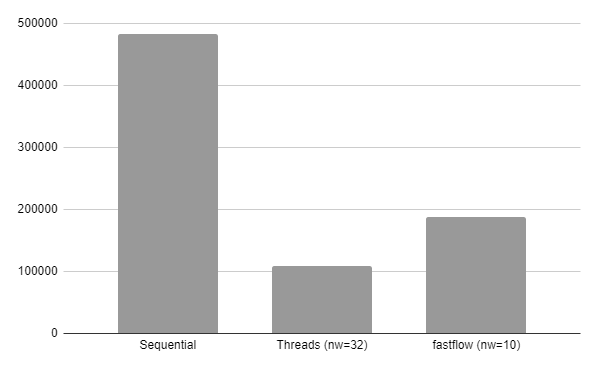
\includegraphics[scale=0.75]{runtimes.png}
\end{center}
\caption{Comparison between the average runtime of the three implementations without file read/write}
\label{figure:runtimes}
\end{figure}
By generating a plot that showcases the average runtime of an implementation in relation to the number of workers employed, we can obtain significant insights into scalability and efficiency. 
\begin{figure}[H]
\begin{center}
	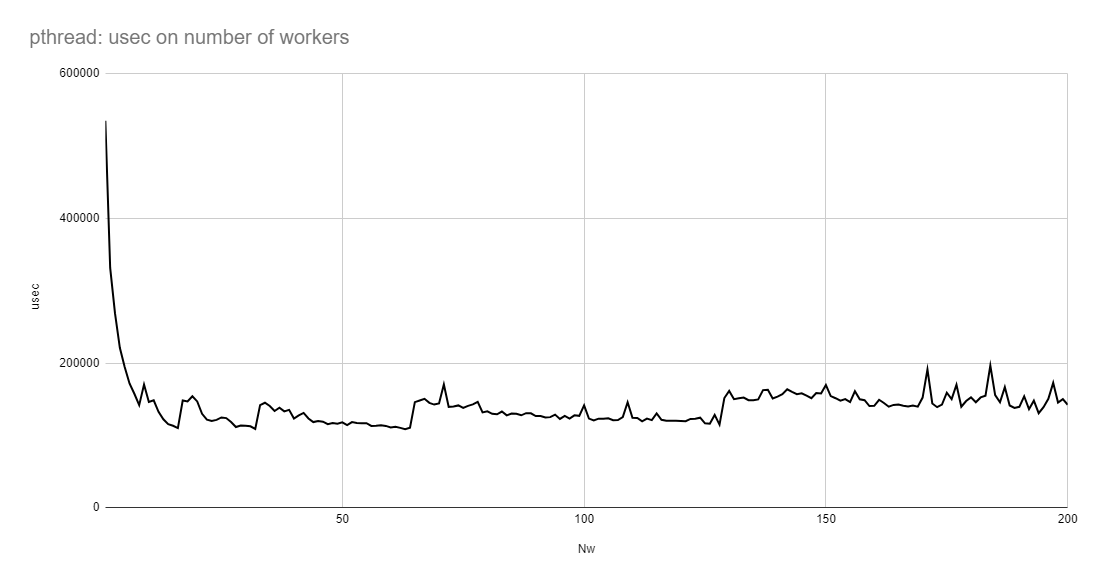
\includegraphics[scale=.6]{scalability_pthreads.png}
\end{center}
\caption{Average execution time of 10 runs over 9M characters per number of workers for the \texttt{pthread} implementation.}
\label{figure:scalability_threads}
\end{figure}
Analyzing the plot depicted in Figure \ref{figure:scalability_threads} for the \texttt{pthread}s implementation, it becomes apparent that the runtime remains relatively stable once the number of workers surpasses a certain threshold (circa 10 workers). This observation suggests that the overhead introduced by data transfers between workers and between pipeline stages has a minimal impact, thereby indicating efficient handling of data within the system. This is further demonstrated by the Table \ref{table:scalability_threads}, showing a scalability value that's comparable across the sampled number of workers\\
The implementation of \texttt{pthread}s is straightforward, involving a fixed-size thread pool and logic for distributing data to and collecting data from the workers in the thread pool. Synchronization mechanisms such as mutexes are employed to ensure proper handling of thread access to shared data, specifically the text portions and heap access. However, the scope of each mutex is minimal, and as indicated by the plot, their impact is negligible, at least until the number of workers reaches 200.\\
The plot reveals a notable pattern characterized by sudden runtime increases occurring every few tens of workers. Although initially appearing random, these jumps consistently occurred at specific worker counts across all experimental runs. The transitions consistently took place from 8 to 9 workers ($2^3 \rightarrow 2^3 + 1$), 16 to 17 workers ($2^4 \rightarrow 2^4 + 1$), 32 to 33 workers ($2^5 \rightarrow 2^5 + 1$), 64 to 65 workers ($2^6 \rightarrow 2^6 + 1$), and 128 to 129 workers ($2^7 \rightarrow 2^7 + 1$). It is reasonable to anticipate a similar jump between 256 and 257 workers and subsequent counts following the same pattern.\\
Considering that these jumps occur precisely at powers of two ($2^n$ workers) and with the compiler optimization flag "-O3" enabling various optimization techniques, it suggests that the optimization methods impact how the system manages threads. It appears that the system utilizes threads more efficiently when employing an exact power of two workers, resulting in improved performance. Conversely, when the worker count falls between $2^{n-1} + 1$ and $2^n - 1$, the runtime performance is slightly compromised, albeit decreasing monotonically.\\
Based on the observed characteristics of the implementation, it is advisable to design a system that utilizes the proposed implementation with a number of workers equal to a power of two. This choice aligns with the fact that the runtime exhibits local minima when the number of workers is a power of two, suggesting that the compiler optimizations are most effectively utilized in such scenarios. By leveraging this knowledge, we can achieve a more efficient utilization of resources and potentially enhance the overall performance of the system.
\begin{figure}[H]
\begin{center}
	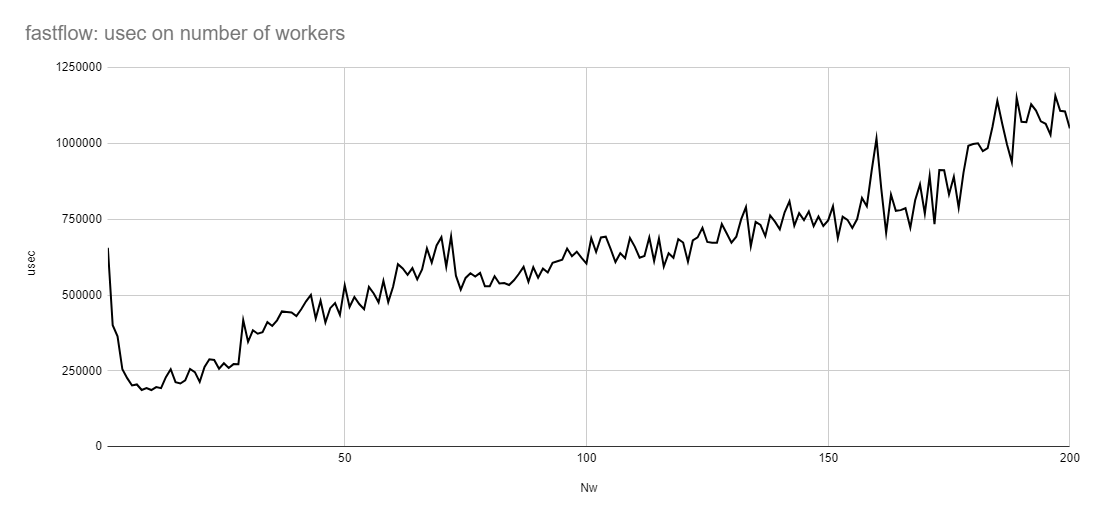
\includegraphics[scale=.6]{scalability_fastflow.png}
\end{center}
\caption{Average execution time of 10 runs over 9M characters per number of workers for the FastFlow implementation.}
\label{figure:Scalability_fastflow}
\end{figure}
The plot in Figure \ref{figure:Scalability_fastflow} clearly demonstrates the key difference between the two implementations: the increasing in runtime as the number of workers increases. In the case of the \texttt{pthread}s implementation, the runtime remains nearly constant, disregarding the previously mentioned pattern of sharp jumps. On the other hand, the FastFlow implementation exhibits a linear increasing in runtime proportional to the number of workers involved.\\
The observed linear increase in runtime in the FastFlow implementation can be attributed to the communication overhead between the nodes of the FastFlow farm and pipeline, as well as between the queues and the nodes themselves. These communication processes contribute to the overall runtime and result in the linear increase in runtime.\\
To further illustrate this behavior, Table \ref{table:scalability_fastflow} provides a numerical representation of the runtime for sampled numbers of workers, with the average runtime recorded. A scalability value less than 1 indicates a degradation in performance, where the runtime exceeds that of running the same algorithm on a single worker. It is important to consider these scalability characteristics when choosing between the \texttt{pthread}s and FastFlow implementations, as they can have a significant impact on the overall performance and efficiency of the system.
%• Should include some discussion relative to the motivation of the differences between achieved performance figures and the ideal/predicted ones, in particular pointing out qualitatively and quantitively, the major sources of overhead.
\pagebreak
\section{Running the Code} 
%• Should include the instructions needed to compile and run the code
The submitted archive contains a \texttt{MakeFile} that handles compilation. Make commands for parallel implementations support a parameter named \texttt{NW} used to specify the number of workers.
\begin{list}{}{}
	\item Sequential program: \texttt{make seq \&\& ./huffman\_seq filename}
	\item \texttt{pthread}s implementation: \texttt{make threads NW=32 \&\& ./huffman\_threads filename}
	\item FastFlow implementation: \texttt{make fastflow NW=10 \&\& ./huffman\_fastflow filename}
\end{list}
\end{document}  
